\documentclass[12pt]{article}

\usepackage{amsmath, mathtools}
\usepackage{amsfonts}
\usepackage{amssymb}
\usepackage{graphicx}
\usepackage{colortbl}
\usepackage{xr}
\usepackage{hyperref}
\usepackage{longtable}
\usepackage{xfrac}
\usepackage{tabularx}
\usepackage{float}
\usepackage{siunitx}
\usepackage{booktabs}
\usepackage{caption}
\usepackage{pdflscape}
\usepackage{afterpage}

\usepackage[round]{natbib}

%\usepackage{refcheck}

\hypersetup{
    bookmarks=true,         % show bookmarks bar?
      colorlinks=true,       % false: boxed links; true: colored links
    linkcolor=red,          % color of internal links (change box color with linkbordercolor)
    citecolor=green,        % color of links to bibliography
    filecolor=magenta,      % color of file links
    urlcolor=cyan           % color of external links
}

%% Comments

\usepackage{color}

\newif\ifcomments\commentsfalse

\ifcomments
\newcommand{\authornote}[3]{\textcolor{#1}{[#3 ---#2]}}
\newcommand{\todo}[1]{\textcolor{red}{[TODO: #1]}}
\else
\newcommand{\authornote}[3]{}
\newcommand{\todo}[1]{}
\fi

\newcommand{\wss}[1]{\authornote{blue}{SS}{#1}} 
\newcommand{\plt}[1]{\authornote{magenta}{TPLT}{#1}} %For explanation of the template
\newcommand{\an}[1]{\authornote{cyan}{Author}{#1}}

%% Common Parts

\newcommand{\progname}{ProgName} % PUT YOUR PROGRAM NAME HERE %Every program
                                % should have a name


% For easy change of table widths
\newcommand{\colZwidth}{1.0\textwidth}
\newcommand{\colAwidth}{0.13\textwidth}
\newcommand{\colBwidth}{0.82\textwidth}
\newcommand{\colCwidth}{0.1\textwidth}
\newcommand{\colDwidth}{0.05\textwidth}
\newcommand{\colEwidth}{0.8\textwidth}
\newcommand{\colFwidth}{0.17\textwidth}
\newcommand{\colGwidth}{0.5\textwidth}
\newcommand{\colHwidth}{0.28\textwidth}

% Used so that cross-references have a meaningful prefix
\newcounter{defnum} %Definition Number
\newcommand{\dthedefnum}{GD\thedefnum}
\newcommand{\dref}[1]{GD\ref{#1}}
\newcounter{datadefnum} %Datadefinition Number
\newcommand{\ddthedatadefnum}{DD\thedatadefnum}
\newcommand{\ddref}[1]{DD\ref{#1}}
\newcounter{theorynum} %Theory Number
\newcommand{\tthetheorynum}{T\thetheorynum}
\newcommand{\tref}[1]{T\ref{#1}}
\newcounter{tablenum} %Table Number
\newcommand{\tbthetablenum}{T\thetablenum}
\newcommand{\tbref}[1]{TB\ref{#1}}
\newcounter{assumpnum} %Assumption Number
\newcommand{\atheassumpnum}{P\theassumpnum}
\newcommand{\aref}[1]{A\ref{#1}}
\newcounter{goalnum} %Goal Number
\newcommand{\gthegoalnum}{P\thegoalnum}
\newcommand{\gsref}[1]{GS\ref{#1}}
\newcounter{instnum} %Instance Number
\newcommand{\itheinstnum}{IM\theinstnum}
\newcommand{\iref}[1]{IM\ref{#1}}
\newcounter{reqnum} %Requirement Number
\newcommand{\rthereqnum}{P\thereqnum}
\newcounter{nfreqnum} %Non-Performance requirement Number
\newcommand{\rthenfreqnum}{P\thenfreqnum}
\newcommand{\rref}[1]{R\ref{#1}}
\newcounter{lcnum} %Likely change number
\newcommand{\lthelcnum}{LC\thelcnum}
\newcommand{\lcref}[1]{LC\ref{#1}}

\usepackage{fullpage}

\begin{document}

\title{Software Requirements Specification for \progname: \
Simulation of a PID control loop.} 
\author{Naveen Ganesh Muralidharan}
\date{\today}
	
\maketitle

~\newpage

\pagenumbering{roman}

\tableofcontents

~\newpage

\section*{Revision History}

\begin{tabularx}{\textwidth}{p{3cm}p{2cm}X}
\toprule {\bf Date} & {\bf Version} & {\bf Notes}\\
\midrule
09-Oct-2020 & 1.0 & A first draft of the SRS\\
12-Oct-2020 & 1.1 & Addressed the following issues,
\begin{itemize}
\item Elaborated Intended reader and user characteristics.
\item Fixed Physical system figure reference.
\item Added reference to assumptions \aref{A_Attn} and \aref{A_Tuning}.
\item Fixed assumption \aref{A_Initial}.
\item Added explanation for system context.
\item Added cross reference in assumptions for readability.
\end{itemize}\\
19-Oct-2020 & 1.2 & Addressed the following issues,
\begin{itemize}
\item Updated the properties of the correct solution and removed the corresponding
non-functional requirement.
\item Rephrased Intended reader characteristics, \ddref{DD_TStep}, and goal statements for
clarity.
\item Added time-domain analysis to the scope.
\item Fixed typographical errors.
\end{itemize}\\
11-Nov-2020 & 1.3 & Addressed the following issues,
\begin{itemize}
\item Removed the second goal statement.
\item Fixed a couple of typos.
\end{itemize}\\
\bottomrule
\end{tabularx}

~\newpage

\section{Reference Material}

This section records information for easy reference.

\subsection{Table of Units}

Throughout this document, SI (Syst\`{e}me International d'Unit\'{e}s) is employed
as the unit system.  In addition to the basic units, several derived units are
used as described below.  For each unit, the symbol is given followed by a
description of the unit and the SI name.
~\newline

\renewcommand{\arraystretch}{1.2}
%\begin{table}[ht]
  \noindent \begin{tabular}{l l l} 
    \toprule		
    \textbf{symbol} & \textbf{unit} & \textbf{SI}\\
    \midrule 
    \si{\second} & time & second\\
    \bottomrule
  \end{tabular}
  %	\caption{Provide a caption}
%\end{table}

\plt{Only include the units that your SRS actually uses.}

\plt{Derived units, like newtons, pascal, etc, should show their derivation
    (the units they are derived from) if their constituent units are in the
    table of units (that is, if the units they are derived from are used in the
    document).  For instance, the derivation of pascals as
    $\si{\pascal}=\si{\newton\per\square\meter}$ is shown if newtons and m are
    both in the table.  The derivations of newtons would not be shown if kg and
    s are not both in the table.}

\plt{The symbol for units named after people use capital letters, but the name
  of the unit itself uses lower case.  For instance, pascals use the symbol Pa,
  watts use the symbol W, teslas use the symbol T, newtons use the symbol N,
  etc.  The one exception to this is degree Celsius.  Details on writing metric
  units can be found on the 
  \href{https://www.nist.gov/pml/weights-and-measures/writing-metric-units}
  {NIST} web-page.}

\subsection{Table of Symbols}

The table that follows summarizes the symbols used in this document along with
their units. The symbols are listed in alphabetical order.

\renewcommand{\arraystretch}{1.2}
%\noindent \begin{tabularx}{1.0\textwidth}{l l X}
\noindent \begin{longtable*}{l l p{9cm}} \toprule
\textbf{symbol} & \textbf{unit} & \textbf{description}\\
\midrule
$e(t)$ & Mathematical value (dimensionless) & Error Signal at time t
\\
$K_d$ & Constant (dimensionless) & Derivative Gain
\\
$K_i$ &  Constant (dimensionless) & Integral Gain
\\
$K_p$ &  Constant (dimensionless) & Proportional Gain
\\
$SP$ & Mathematical value (dimensionless) & Set Point
\\
$T_\text{sim}$ & \si[per-mode=symbol] {\second} & Total Simulation Time
\\
$T_\text{elapsed}$ & \si[per-mode=symbol] {\second} & Elapsed time
\\
$T_\text{now}$ & \si[per-mode=symbol] {\second} & Time point now
\\ 
$T_\text{prev}$ & \si[per-mode=symbol] {\second} & Previous time point
\\
$t_\text{step}$ & \si[per-mode=symbol] {\second} & Simulation step time
\\
$u(t)$ & Mathematical value (dimensionless) & Control Variable at time t
\\
$x(t)$ & Mathematical value (dimensionless) & A generic input signal at time t
\\
$y(t)$ & Mathematical value (dimensionless) & Process Variable at time t
\\ 
\bottomrule
\end{longtable*}
\plt{Use your problems actual symbols.  The si package is a good idea to use for
  units.}

\subsection{Abbreviations and Acronyms}

\renewcommand{\arraystretch}{1.2}
\begin{tabular}{l l} 
  \toprule		
  \textbf{symbol} & \textbf{description}\\
  \midrule 
  A & Assumption\\
  API & Application Program Interface\\
  CV & Control Variable\\
  D & Derivative term of the PID controller\\
  DD & Data Definition\\
  etc & Et cetera\\
  GD & General Definition\\
  GS & Goal Statement\\
  I & Integral term of the PID controller\\
  IM & Instance Model\\
  LC & Likely Change\\
  P & Proportional term of the PID controller\\
  PID & Proportional Integral Derivative\\
  PS & Physical System Description\\
  PV & Process Variable\\
  R & Requirement\\
  SP & Set Point\\
  SRS & Software Requirements Specification\\
  T & Theoretical Model\\
  \bottomrule
\end{tabular}\\

\plt{Add any other abbreviations or acronyms that you add}

\newpage

\pagenumbering{arabic}

\plt{This SRS template is based on \citet{SmithAndLai2005, SmithEtAl2007}.  It
  will get you started.  You should not modify the section headings, without
  first discussing the change with the course instructor.  Modification means
  you are not following the template, which loses some of the advantage of a
  template, especially standardization.  Although the bits shown below do not
  include type information, you may need to add this information for your
  problem.  If you are unsure, please can ask the instructor.}

\plt{Feel free to change the appearance of the report by modifying the LaTeX
  commands.}

\plt{This template document assumes that a single program is being documented.
  If you are documenting a family of models, you should start with a commonality
  analysis.  A separate template is provided for this.  For program
  families you should look at \cite{Smith2006, SmithMcCutchanAndCarette2017}.
  Single family member programs are often programs based on a single physical
  model.  General purpose tools are usually documented as a family.  Families of
  physical models also come up.}

\plt{The SRS is not generally written, or read, sequentially.  The SRS is a
  reference document.  It is generally read in an ad hoc order, as the need
  arises.  For writing an SRS, and for reading one for the first time, the
  suggested order of sections is:
\begin{itemize}
\item Goal Statement
\item Instance Models
\item Requirements
\item Introduction
\item Specific System Description
\end{itemize}
}

\plt{Guiding principles for the SRS document:
\begin{itemize}
\item Do not repeat the same information at the same abstraction level.  If
  information is repeated, the repetition should be at a different abstraction
  level.  For instance, there will be overlap between the scope section and the
  assumptions, but the scope section will not go into as much detail as the
  assumptions section.
\end{itemize}
}

\plt{The template description comments should be disabled before submitting this
  document for grading.}

\plt{You can borrow any wording from the text given in the template.  It is part
  of the template, and not considered an instance of academic integrity.  Of
  course, you need to cite the source of the template.}

\plt{When the documentation is done, it should be possible to trace back to the
  source of every piece of information.  Some information will come from
  external sources, like terminology.  Other information will be derived, like
  General Definitions.}

\plt{An SRS document should have the following qualities: unambiguous,
  consistent, complete, validatable, abstract and traceable.}

\plt{The overall goal of the SRS is that someone that meets the Characteristics
  of the Intended Reader (Section~\ref{sec_IntendedReader}) can learn,
  understand and verify the captured domain knowledge.  They should not have to
  trust the authors of the SRS on any statements.  They should be able to
  independently verify/derive every statement made.}

\section{Introduction}

\plt{The introduction section is written to introduce the problem.  It starts
  general and focuses on the problem domain. The general advice is to start with
a paragraph or two that describes the problem, followed by a ``road-map''
paragraph.  A road-map orients the reader by telling them what sub-sections to
expect in the Introduction section.}

A closed loop control system with a PID controller is used in a wide range of 
applications such as a thermostat, automobile cruise-control, etc. The 
gains of a PID controller in an application must be tuned before the 
controller is ready for production. Therefore, a software model is necessary for 
the simulation of PID controller.

~\newline
In this section, the purpose of the document is first discussed, followed by the
scope of the requirements, characteristics of the intended reader, and finally the 
organization of the document.

\subsection{Purpose of Document}

\plt{This section summarizes the purpose of the SRS document.  It does not focus
  on the problem itself.  The problem is described in the ``Problem
  Description'' section (Section~\ref{Sec_pd}).  The purpose is for the document
  in the context of the project itself, not in the context of the CAS 741
  course.  Although the ``purpose'' of the document is to get a grade in 741,
  you should not mention this.  Instead, ``fake it'' as if this is a real
  project.  The purpose section will be similar between projects.  The purpose
  of the document is the purpose of the SRS, including communication, planning
  for the design stage, etc.}

The purpose of this document is to capture all the necessary information
including assumptions, data definitions, constraints, models, and 
requirements to facilitate an unambiguous development of the PID controller 
software and test procedures.

\subsection{Scope of Requirements} 

\plt{Modelling the real world requires simplification.  The full complexity of
  the actual physics, chemistry, biology is too much for existing models, and
  for existing computational solution techniques.  Rather than say what is in
  the scope, it is usually easier to say what is not.  You can think of it as
  the scope is initially everything, and then it is constrained to create the
  actual scope.  For instance, the problem can be restricted to 2 dimensions, or
  it can ignore the effect of temperature (or pressure) on the material
  properties, etc.}  

\plt{The scope section is related to the assumptions section
  (Section~\ref{sec_assumpt}).  However, the scope and the assumptions are not
  at the same level of abstraction.  The scope is at a high level.  The focus is
  on the ``big picture'' assumptions.  The assumptions section lists, and
  describes, all of the assumptions.}
  
The scope of the requirements is limited to the simulation of a closed
loop control system with three subsystems, namely, a Summing point, a PID 
controller, and a Power Plant. All the analyses  in this application are in the 
time domain.

\subsection{Characteristics of Intended Reader} \label{sec_IntendedReader}

\plt{This section summarizes the skills and knowledge of the readers of the
  SRS.  It does NOT have the same purpose as the ``User Characteristics''
  section (Section~\ref{SecUserCharacteristics}).  The intended readers are the
  people that will read, review and maintain the SRS.  They are the people that
  will conceivably design the software that is intended to meet the
  requirements.  The user, on the other hand, is the person that uses the
  software that is built.  They may never read this SRS document.  Of course,
  the same person could be a ``user'' and an ``intended reader.''}

\plt{The intended reader characteristics should be written as unambiguously and
  as specifically as possible.  Rather than say, the user should have an
  understanding of physics, say what kind of physics and at what level.  For
  instance, is high school physics adequate, or should the reader have had a
  graduate course on advanced quantum mechanics?}

The reader of this document is assumed to have prerequisite knowledge of 
Control System (Control theory and controllers) at a fourth-year undergraduate 
engineering level, and knowledge of calculus at the high school level. 

\subsection{Organization of Document}

\plt{This section provides a roadmap of the SRS document.  It will help the
  reader orient themselves.  It will provide direction that will help them
  select which sections they want to read, and in what order.  This section will
  be similar between project.}

The sections in this document are based on \citet{SmithAndLai2005, 
SmithEtAl2007}. Subsequent sections of this document will breakdown and present 
the problem in a less abstract manner than the previous section. 
For example, the context for the mathematical equations required to solve the 
problem is set in the Theoretical Models and are refined in General and Data 
Definitions and the final form of the equations are derived in the Instance 
Models. 

~\newline
The suggested order of reading this document for a reader who is not familiar 
with the domain would be to start with the problem description, review goals, 
and proceed to the subsequent sections. A reader with knowledge of the domain 
can directly review the Instance Models and choose to proceed in either direction.

\section{General System Description}

This section provides general information about the system. It identifies the
interfaces between the system and its environment, describes the user
characteristics, and lists the system constraints.  \plt{This text can likely be
  borrowed verbatim.}

\plt{The purpose of this section is to provide general information about the
  system so the specific requirements in the next section will be easier to
  understand. The general system description section is designed to be
  changeable independent of changes to the functional requirements documented in
  the specific system description. The general system description provides a
  context for a family of related models.  The general description can stay the
  same, while specific details are changed between family members.}

\subsection{System Context}

\plt{Your system context will include a figure that shows the abstract view of
  the software.  Often in a scientific context, the program can be viewed
  abstractly following the design pattern of Inputs $\rightarrow$ Calculations
  $\rightarrow$ Outputs.  The system context will therefore often follow this
  pattern.  The user provides inputs, the system does the calculations, and then
  provides the outputs to the user.  The figure should not show all of the
  inputs, just an abstract view of the main categories of inputs (like material
  properties, geometry, etc.).  Likewise, the outputs should be presented from
  an abstract point of view.  In some cases the diagram will show other external
  entities, besides the user.  For instance, when the software product is a
  library, the user will be another software program, not an actual end user.}

Figure-\ref{Fig_SystemContext} shows the system context. The circle represents an
external entity outside the software, the user in this case. The rectangle  represents the 
software system itself, the PID Control Loop in this case.  Arrows are used to show the 
data between the system and its environment.

\begin{figure}[h!]
\begin{center}
 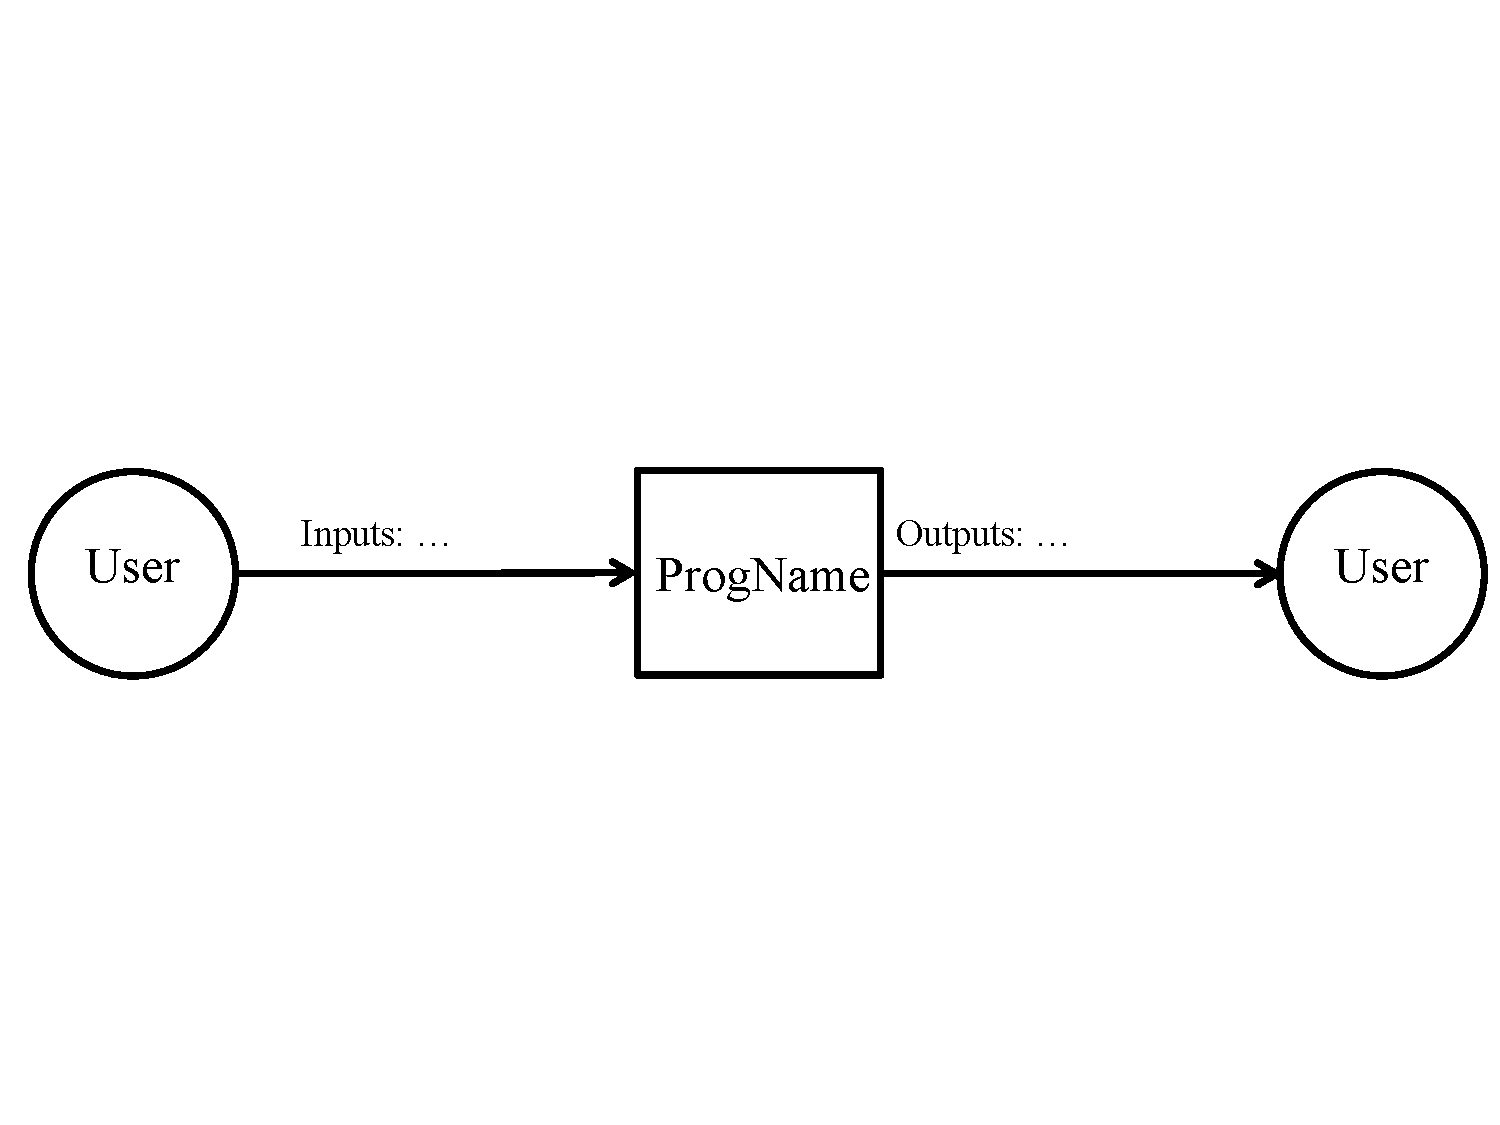
\includegraphics[width=0.7\textwidth]{SystemContextFigure}
\caption{System Context}
\label{Fig_SystemContext} 
\end{center}
\end{figure}

\plt{For each of the entities in the system context diagram its responsibilities
  should be listed.  Whenever possible the system should check for data quality,
  but for some cases the user will need to assume that responsibility.}

The PID controller is self-contained. The only external interaction is with the 
user. The responsibilities of the user and the system are as follows,

\begin{itemize}
\label{sec_User_Responsibilities}
\item User Responsibilities:
\begin{itemize}
\item Feed inputs to the model.
\item Review the response of the Power-Plant.
\item Tune the controller gains.
\end{itemize}
\item \progname{} Responsibilities:
\begin{itemize}
\item Calculate the outputs of the PID controller and Power Plant.
\end{itemize}
\end{itemize}

\subsection{User Characteristics} \label{SecUserCharacteristics}

\plt{This section summarizes the knowledge/skills expected of the user.
  Measuring usability, which is often a required non-function requirement,
  requires knowledge of a typical user.  As mentioned above, the user is a
  different role from the ``intended reader,'' as given in
  Section~\ref{sec_IntendedReader}.  As in Section~\ref{sec_IntendedReader}, the
  user characteristics should be specific an unambiguous.  For instance, ``The
  end user of \progname{} should have an understanding of undergraduate Level 1
  Calculus and Physics.''}
  
The end-user of \progname{} should at the minimum have knowledge of Control 
Systems at a second-year undergraduate engineering level, and knowledge 
of High school Calculus.

\subsection{System Constraints}

\plt{System constraints differ from other type of requirements because they
  limit the developers’ options in the system design and they identify how the
  eventual system must fit into the world. This is the only place in the SRS
  where design decisions can be specified.  That is, the quality requirement for
  abstraction is relaxed here.  However, system constraints should only be
  included if they are truly required. In the context of CAS 741, you often will
  may not have any system constraints.}

%\subsection{System Constraints}

\plt{System constraints differ from other type of requirements because they
  limit the developers’ options in the system design and they identify how the
  eventual system must fit into the world. This is the only place in the SRS
  where design decisions can be specified.  That is, the quality requirement for
  abstraction is relaxed here.  However, system constraints should only be
  included if they are truly required. In the context of CAS 741, you often will
  may not have any system constraints.}
   
No system constraints were identified for \progname{}.

\section{Specific System Description}

This section first presents the problem description, which gives a high-level
view of the problem to be solved.  This is followed by the solution characteristics
specification, which presents the assumptions, theories, definitions, and finally
the instance models.  \plt{Add any project specific details that are relevant
  for the section overview.}

\subsection{Problem Description} \label{Sec_pd}

This program intends to provide a model of a PID controller that can be used 
for the tuning of the gain constants before the deployment of the controller.

\subsubsection{Terminology and  Definitions}

\plt{This section is expressed in words, not with equations.  It provide the
  meaning of the different words and phrases used in the domain of the problem.
The terminology is used to introduce concepts from the world outside of the
mathematical model  The terminology provides a real world connection to give the
mathematical model meaning.}

This subsection provides a list of terms which are used in the subsequent
sections and their meaning, with the purpose of reducing ambiguity and making it
easier to correctly understand the requirements:

\begin{itemize}

\item [Control Variable:] The output from the PID controller.

\item [Error Value:] Input to the PID controller. Error Value is the 
difference between the Set Point and the Process Variable. 

\item [Elapsed Time:] Time elapsed between subsequent iterations of the control
loop.

\item [PID Control Loop:] Closed loop control system with PID Controller, 
Summing Point, and Power Plant.

\item [Power Plant:] The system to be controlled. 

\item [Process Variable:] The output value from the power plant.

\item [Set-Point:] The desired value that the control system must reach.

\item [Simulation Time:] Total execution time of the application.

\item [Step Time:] Optimal wait time for one iteration of the control loop.

\item [Summing Point:] Control block where the difference between the Set-Point
and the Process Variable is computed. 

\end{itemize}

\subsubsection{Physical System Description} \label{sec_phySystDescrip}

\plt{The purpose of this section is to clearly and unambiguously state the
  physical system that is to be modelled. Effective problem solving requires a
  logical and organized approach. The statements on the physical system to be
  studied should cover enough information to solve the problem. The physical
  description involves element identification, where elements are defined as
  independent and separable items of the physical system. Some example elements
  include acceleration due to gravity, the mass of an object, and the size and
  shape of an object. Each element should be identified and labelled, with their
  interesting properties specified clearly. The physical description can also
  include interactions of the elements, such as the following: i) the
  interactions between the elements and their physical environment; ii) the
  interactions between elements; and, iii) the initial or boundary conditions.}

The physical system of a PID control loop, as shown in Figure-\ref{fig_PID_Control},
includes the following elements:

\begin{itemize}

\item[PS1:] Summing Point

\item[PS2:] PID Controller 

\item[PS3:] Power Plant

\end{itemize}

\plt{A figure here makes sense for most SRS documents}

\begin{figure}[h!]
\begin{center}
%\rotatebox{-90}
{
 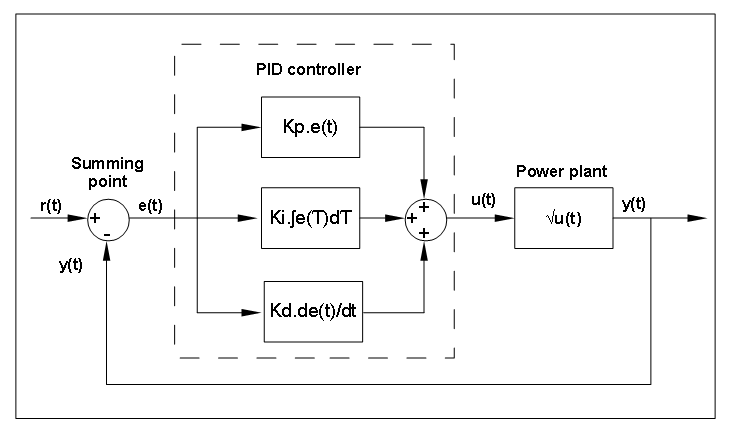
\includegraphics[width=0.9\textwidth]{Fig_PIDController.png}
}
\caption{\label{fig_PID_Control} PID Control Loop}
\end{center}
\end{figure}

\subsubsection{Goal Statements}

\plt{The goal statements refine the ``Problem Description''
  (Section~\ref{Sec_pd}).  A goal is a functional objective the system under
  consideration should achieve. Goals provide criteria for sufficient
  completeness of a requirements specification and for requirements
  pertinence. Goals will be refined in Section “Instanced Models”
  (Section~\ref{sec_instance}). Large and complex goals should be decomposed
  into smaller sub-goals.  The goals are written abstractly, with a minimal
  amount of technical language.  They should be understandable by non-domain
  experts.}

\noindent Given the Set-Point, Proportional Gain, Integral Gain, Derivative Gain, 
Total Simulation time, and Step Time, the goal statements are:

\begin{itemize}
% \item[GS\refstepcounter{goalnum}\thegoalnum \label{G_ES}:] \plt{One
    % sentence description of the goal.  There may be more than one.  Each Goal
    % should have a meaningful label.}
	% Calculate the Error-Value at every step.

% \item[GS\refstepcounter{goalnum}\thegoalnum \label{G_CV}:] Compute the 
% output of the PID-controller at every step.

\item[GS\refstepcounter{goalnum}\thegoalnum \label{G_PV}:] Compute the 
output (Process Variable) of the Power-Plant at every step.


\end{itemize}

\subsection{Solution Characteristics Specification}

\plt{This section specifies the information in the solution domain of the system
  to be developed. This section is intended to express what is required in
  such a way that analysts and stakeholders get a clear picture, and the
  latter will accept it. The purpose of this section is to reduce the problem
  into one expressed in mathematical terms. Mathematical expertise is used to
  extract the essentials from the underlying physical description of the
  problem, and to collect and substantiate all physical data pertinent to the
  problem.}

\plt{This section presents the solution characteristics by successively refining
  models.  It starts with the abstract/general Theoretical Models (TMs) and
  refines them to the concrete/specific Instance Models (IMs).  If necessary
  there are intermediate refinements to General Definitions (GDs).  All of these
  refinements can potentially use Assumptions (A) and Data Definitions (DD).
  TMs are refined to create new models, that are called GMs or IMs. DDs are not
  refined; they are just used. GDs and IMs are derived, or refined, from other
  models. DDs are not derived; they are just given. TMs are also just given, but
  they are refined, not used.  If a potential DD includes a derivation, then
  that means it is refining other models, which would make it a GD or an IM.}

\plt{The above makes a distinction between ``refined'' and ``used.'' A model is
  refined to another model if it is changed by the refinement. When we change a
  general 3D equation to a 2D equation, we are making a refinement, by applying
  the assumption that the third dimension does not matter. If we use a
  definition, like the definition of density, we aren't refining, or changing
  that definition, we are just using it.}

\plt{The same information can be a TM in one problem and a DD in another.  It is
  about how the information is used.  In one problem the definition of
  acceleration can be a TM, in another it would be a DD.}

\plt{There is repetition between the information given in the different chunks
  (TM, GDs etc) with other information in the document.  For instance, the
  meaning of the symbols, the units etc are repeated.  This is so that the
  chunks can stand on their own when being read by a reviewer/user.  It also
  facilitates reuse of the models in a different context.}

\noindent \plt{The relationships between the parts of the document are show in
  the following figure.  In this diagram ``may ref'' has the same role as
  ``uses'' above.  The figure adds ``Likely Changes,'' which are able to
  reference (use) Assumptions.}

\begin{figure}[H]
  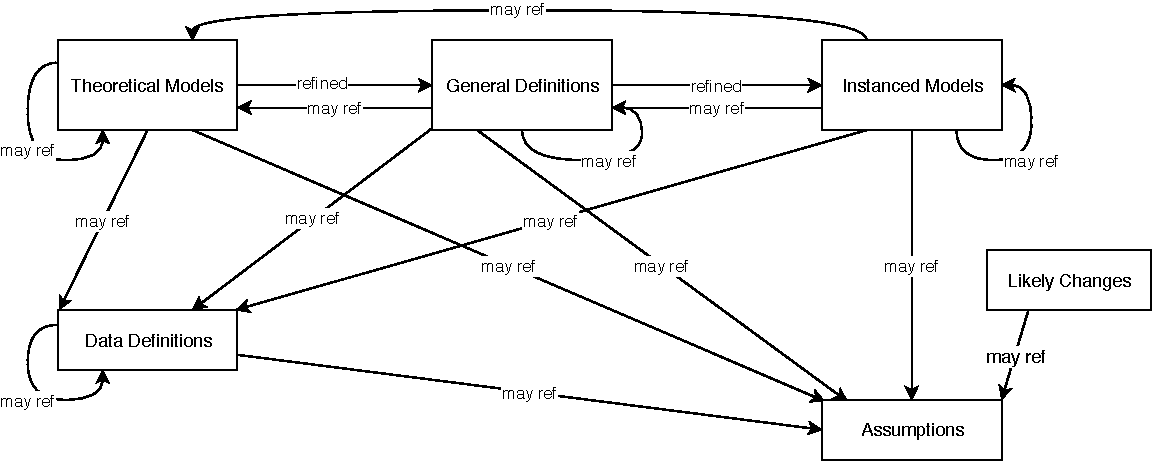
\includegraphics[scale=0.9]{RelationsBetweenTM_GD_IM_DD_A.pdf}
\end{figure}

The instance models that govern \progname{} are presented in
Subsection~\ref{sec_instance}.  The information to understand the meaning of the
instance models and their derivation is also presented so that the instance
models can be verified.

\subsubsection{Assumptions} \label{sec_assumpt}

\plt{The assumptions are a refinement of the scope.  The scope is general, where
  the assumptions are specific.  All assumptions should be listed, even those
  that domain experts know so well that they are rarely (if ever) written down.}
\plt{The document should not take for granted that the reader knows which
  assumptions have been made. In the case of unusual assumptions, it is
  recommended that the documentation either include, or point to, an explanation
  and justification for the assumption.}

This section simplifies the original problem and helps in developing the
theoretical model by filling in the missing information for the physical
system. The numbers given in the square brackets refer to the theoretical model
[T], general definition [GD], data definition [DD], instance model [IM], or
likely change [LC], in which the respective assumption is used.

\begin{itemize}

\item[A\refstepcounter{assumpnum}\theassumpnum \label{A_PP}:]
  \plt{Short description of each assumption.  Each assumption
    should have a meaningful label.  Use cross-references to identify the
    appropriate traceability to T, GD, DD etc., using commands like dref, ddref
    etc.  Each assumption should be atomic - that is, there should not be an
    explicit (or implicit) ``and'' in the text of an assumption.}
	
    Contrary to the real world, the Power Plant and the Sensor are coupled 
    into a single system, with a response of $f(x) = \sqrt{x}$ [Ref By: 
    \iref{IM_EV}, \lcref{LC_PP}].

\item[A\refstepcounter{assumpnum}\theassumpnum \label{A_EQ}:] This program uses
 the decoupled form of the equation of the PID controller [Ref By: \iref{IM_CV}, 
    \lcref{LC_EQ}].

\item[A\refstepcounter{assumpnum}\theassumpnum \label{A_SP}:] The Set-Point is 
constant throughout the execution of the program [Ref By: \ddref{DD_SP}, 
    \lcref{LC_SP}].

\item[A\refstepcounter{assumpnum}\theassumpnum \label{A_Attn}:] There are no 
external disturbances to the Power plant during the simulation [\cite{PID_Wiki}]
[Ref By: \iref{IM_PV}].

\item[A\refstepcounter{assumpnum}\theassumpnum \label{A_Delay}:] There are no 
delays in the signal propagation, other than the step time,
during the simulation [\cite{PID_Wiki}] [Ref By: \ddref{DD_TStep}].

\item[A\refstepcounter{assumpnum}\theassumpnum \label{A_Tuning}:] This model 
will be used for the Manual tuning of the control gains by the user 
[Ref By: \ddref{DD_Proportional}, \ddref{DD_Integ}, \ddref{DD_Derivative}].

\item[A\refstepcounter{assumpnum}\theassumpnum \label{A_Initial}:] The initial
value (at the start of the simulation) of the Process Variable is assumed to be 
zero [Ref By: \iref{IM_EV}, \lcref{LC_Initial}].

\item[A\refstepcounter{assumpnum}\theassumpnum \label{A_Parallel}:] The Parallel
form of the equation is used for the PID controller 
[Ref By: \iref{IM_CV}, \lcref{LC_U_Parallel}].

\end{itemize}

\subsubsection{Theoretical Models}\label{sec_theoretical}

\plt{Theoretical models are sets of abstract mathematical equations or axioms
  for solving the problem described in Section ``Physical System Description''
  (Section~\ref{sec_phySystDescrip}). Examples of theoretical models are
  physical laws, constitutive equations, relevant conversion factors, etc.}

This section focuses on the general equations and laws that the application is 
based on.  \plt{Modify the examples below for your problem, and add additional 
models as appropriate.}
  
~\newline \progname{} is not based on any general equation or laws.


\subsubsection{General Definitions}\label{sec_gendef}

\plt{General Definitions (GDs) are a refinement of one or more TMs, and/or of
  other GDs.  The GDs are less abstract than the TMs.  Generally the reduction
  in abstraction is possible through invoking (using/referencing) Assumptions.
  For instance, the TM could be Newton's Law of Cooling stated abstracting.  The
  GD could take the general law and apply it to get a 1D equation.}

This section collects the laws and equations that will be used in building the
instance models. 

~\newline This section is not applicable to  \progname{}.

\plt{Some projects may not have any content for this section, but the section
  heading should be kept.}  \plt{Modify the examples below for your problem, and
  add additional definitions as appropriate.}

\plt{This may be necessary when the necessary information does not fit in the
  description field.}
\plt{Derivations are important for justifying a given GD.  You want it to be
  clear where the equation came from.}

\subsubsection{Data Definitions}\label{sec_datadef}

\plt{The Data Definitions are definitions of symbols and equations that are
  given for the problem.  They are not derived; they are simply used by other
  models.  For instance, if a problem depends on density, there may be a data
  definition for the equation defining density.  The DDs are given information
  that you can use in your other modules.}

\plt{All Data Definitions should be used (referenced) by at least one other
  model.}

This section collects and defines all the data needed to build the instance
models. The dimension of each quantity is also given.  \plt{Modify the examples
  below for your problem, and add additional definitions as appropriate.}

~\newline

\noindent
\begin{minipage}{\textwidth}
\renewcommand*{\arraystretch}{1.5}
\begin{tabular}{| p{\colAwidth} | p{\colBwidth}|}
\hline
\rowcolor[gray]{0.9}
Number& DD\refstepcounter{datadefnum}\thedatadefnum \label{DD_SP}\\
\hline
Label& \bf Set Point\\
\hline
Symbol &$SP$\\
\hline
% Units& -$\\
% \hline
  SI Units & -\\
  \hline
  Equation& - \\
  \hline
  Description & 
  The Set Point (SP) is the expected output that the control loop must achieve.
  For this simulation, the set-point is assumed to be constant throughout the 
  simulation (\aref{A_SP}).
  \\
  \hline
  Source &
  \cite{PID_Control} \\
  \hline
  Ref.\ By & \iref{IM_EV}\\
  \hline
\end{tabular}
\end{minipage}\\


~\newline

\noindent
\begin{minipage}{\textwidth}
\renewcommand*{\arraystretch}{1.5}
\begin{tabular}{| p{\colAwidth} | p{\colBwidth}|}
\hline
\rowcolor[gray]{0.9}
Number& DD\refstepcounter{datadefnum}\thedatadefnum \label{DD_Proportional}\\
\hline
Label& \bf Proportional term\\
\hline
Symbol &$P$\\
\hline
% Units& -$\\
% \hline
  SI Units & -\\
  \hline
  Equation& $P$ = $K_p$ . $x(t)$ \\
  \hline
  Description & 
  The proportional term of the PID controller is the product of the input 
  ($x(t)$) and the proportional gain $K_p$. $K_p$ is tuned by the user
  (\aref{A_Tuning}).
  \\
  \hline
  Source &
  \cite{PID_Control} \\
  \hline
  Ref.\ By & \iref{IM_CV}\\
  \hline
\end{tabular}
\end{minipage}\\

~\newline

\noindent
\begin{minipage}{\textwidth}
\renewcommand*{\arraystretch}{1.5}
\begin{tabular}{| p{\colAwidth} | p{\colBwidth}|}
\hline
\rowcolor[gray]{0.9}
Number& DD\refstepcounter{datadefnum}\thedatadefnum \label{DD_Integ}\\
\hline
Label& \bf Integral term\\
\hline
Symbol &$I$\\
\hline
% Units& -$\\
% \hline
  SI Units & -\\
  \hline
  Equation& $I$ = $K_i$ . $\int_{0}^{t} x(\tau) d\tau $ \\
  \hline
  Description & 
  The integral term of the PID controller is a product of the accumulated input 
  over time and the integral gain $K_i$. $K_i$ is tuned by the user
  (\aref{A_Tuning}).
  \\
  \hline
  Source &
  \cite{PID_Control} \\
  \hline
  Ref.\ By & \iref{IM_CV}\\
  \hline
\end{tabular}
\end{minipage}\\

~\newline

\noindent
\begin{minipage}{\textwidth}
\renewcommand*{\arraystretch}{1.5}
\begin{tabular}{| p{\colAwidth} | p{\colBwidth}|}
\hline
\rowcolor[gray]{0.9}
Number& DD\refstepcounter{datadefnum}\thedatadefnum \label{DD_Derivative}\\
\hline
Label& \bf Derivative term\\
\hline
Symbol &$D$\\
\hline
% Units& -$\\
% \hline
  SI Units & -\\
  \hline
  Equation& $D$ = $K_d$ . $\frac{d(x(t))}{dt}$ \\
  \hline
  Description & 
  The derivative term of the PID controller is a product of the rate of change
  of the input and the derivative constant $K_d$. $K_d$ is tuned by the user
  (\aref{A_Tuning}).
  \\
  \hline
  Source &
  \cite{PID_Control} \\
  \hline
  Ref.\ By & \iref{IM_CV}\\
  \hline
\end{tabular}
\end{minipage}\\

~\newline

\noindent
\begin{minipage}{\textwidth}
\renewcommand*{\arraystretch}{1.5}
\begin{tabular}{| p{\colAwidth} | p{\colBwidth}|}
\hline
\rowcolor[gray]{0.9}
Number& DD\refstepcounter{datadefnum}\thedatadefnum \label{DD_TSim}\\
\hline
Label& \bf Total Simulation time \\
\hline
Symbol &$T_\text{sim}$\\
\hline
% Units& s\\
% \hline
  SI Units & second\\
  \hline
  Equation& - \\
  \hline
  Description & 
  $T_\text{sim}$ is the total time that the control loop must execute. This
  is required to terminate the execution in case the Power-Plant is in an 
  unstable state (oscillation).
  \\
  \hline
  Source &
  - \\
  \hline
  Ref.\ By & \rref{R_SimTime}\\
  \hline
\end{tabular}
\end{minipage}\\

~\newline

\noindent
\begin{minipage}{\textwidth}
\renewcommand*{\arraystretch}{1.5}
\begin{tabular}{| p{\colAwidth} | p{\colBwidth}|}
\hline
\rowcolor[gray]{0.9}
Number& DD\refstepcounter{datadefnum}\thedatadefnum \label{DD_TStep}\\
\hline
Label& \bf Simulation step time \\
\hline
Symbol &$t_\text{step}$\\
\hline
% Units& s\\
% \hline
  SI Units & second\\
  \hline
  Equation& - \\
  \hline
  Description & 
  $t_\text{step}$ is a time between consecutive iterations of the control loop.
  This is equivalent to the sum of all the delays (from Controller, Power-Plant and sensor) in the real world (\aref{A_Delay}).
  \\
  \hline
  Source &
  - \\
  \hline
  Ref.\ By & \rref{R_SimTime}\\
  \hline
\end{tabular}
\end{minipage}\\

~\newline

\noindent
\begin{minipage}{\textwidth}
\renewcommand*{\arraystretch}{1.5}
\begin{tabular}{| p{\colAwidth} | p{\colBwidth}|}
\hline
\rowcolor[gray]{0.9}
Number& DD\refstepcounter{datadefnum}\thedatadefnum \label{DD_TN}\\
\hline
Label& \bf Time Point Now \\
\hline
Symbol &$T_\text{now}$\\
\hline
% Units& s\\
% \hline
  SI Units & second\\
  \hline
  Equation& - \\
  \hline
  Description & 
  $T_\text{now}$ is the time elapsed since epoch in seconds.
  \\
  \hline
  Source &
  - \\
  \hline
  Ref.\ By & \iref{IM_ET} \ddref{DD_TPrev} \\
  \hline
\end{tabular}
\end{minipage}\\

~\newline

\noindent
\begin{minipage}{\textwidth}
\renewcommand*{\arraystretch}{1.5}
\begin{tabular}{| p{\colAwidth} | p{\colBwidth}|}
\hline
\rowcolor[gray]{0.9}
Number& DD\refstepcounter{datadefnum}\thedatadefnum \label{DD_TPrev}\\
\hline
Label& \bf Previous Time Point \\
\hline
Symbol & $T_\text{prev}$\\
\hline
% Units& s\\
% \hline
  SI Units & second\\
  \hline
  Equation& - \\
  \hline
  Description & 
  $T_\text{prev}$ is the last calculated value of Time Point (from \ddref{DD_TN}).
  \\
  \hline
  Source &
  - \\
  \hline
  Ref.\ By & \iref{IM_ET}\\
  \hline
\end{tabular}
\end{minipage}\\

\subsubsection{Instance Models} \label{sec_instance}    

\plt{The motivation for this section is to reduce the problem defined in
  ``Physical System Description'' (Section~\ref{sec_phySystDescrip}) to one
  expressed in mathematical terms. The IMs are built by refining the TMs and/or
  GDs.  This section should remain abstract.  The SRS should specify the
  requirements without considering the implementation.}

This section transforms the problem defined in Section~\ref{Sec_pd} into 
one which is expressed in mathematical terms. It uses concrete symbols defined 
in Section~\ref{sec_datadef} to replace the abstract symbols in the models 
identified in Sections~\ref{sec_theoretical} and~\ref{sec_gendef}.

~\newline Goal \ref{G_PV} is solved by \iref{IM_PV} and \iref{IM_ET}.

\plt{reference your instancemodels.}  \plt{other details, with cross-references where appropriate.} \plt{Modify the examples below for your problem, and add additional models as appropriate.}

~\newline

%Instance Model 1

\noindent
\begin{minipage}{\textwidth}
\renewcommand*{\arraystretch}{1.5}
\begin{tabular}{| p{\colAwidth} | p{\colBwidth}|}
  \hline
  \rowcolor[gray]{0.9}
  Number& IM\refstepcounter{instnum}\theinstnum \label{IM_EV}\\
  \hline
  Label& \bf Calculate the error signal, $e(t)$\\
  \hline
  Input& $SP$ (\ddref{DD_SP}), $y(t)$ (\iref{IM_PV}) 
  ~\newline The initial value of the process variable, $y(t)$, is assumed to be 
  zero (\aref{A_Initial}).\\
  \hline
  Output & $e(t)$, such that $e(t)$ = $SP$ - $y(t)$\\
  \hline
  Description & The error term is the difference between the Set-Point (required
  value), and Process Variable, (the measured value). The error term is 
  calculated at each step of the simulation.\\
  \hline
  Sources& 
  \cite{PID_Control} \\
  \hline
  Ref.\ By & \iref{IM_CV} \rref{R_Calculate}\\
  \hline
\end{tabular}
\end{minipage}\\

~\newline

%Instance Model 2
\noindent
\begin{minipage}{\textwidth}
\renewcommand*{\arraystretch}{1.5}
\begin{tabular}{| p{\colAwidth} | p{\colBwidth}|}
  \hline
  \rowcolor[gray]{0.9}
  Number& IM\refstepcounter{instnum}\theinstnum \label{IM_CV}\\
  \hline
  Label& \bf Calculate the control variable, $u(t)$\\
  \hline
  Input& $e(t)$ (\iref{IM_EV})\\
  \hline
  Output & $u(t)$, such that $u(t)$ = $K_p$ . $e(t)$ +  $K_i$ . $\int_{0}^{t} 
  e(\tau) d\tau$ + $K_d$ . $\frac{d(e(t))}{dt}$ \\
  \hline
  Description & The Control Variable, $u(t)$ is the output of the PID controller.
  The Control Variable is the sum of the  present (Proportional), past (Integral) 
  and future (Derivative) values of the error. The control variable is 
  calculated at each step of the simulation. The equation used for the PID 
  controller is parallel (\aref{A_Parallel}), that is, the P, I, D components are parallel
   to each other, and de-coupled (\aref{A_EQ}), that is the gains of 
  the P, I, D component are not inter-dependent.\\
  \hline
  Sources& 
  \cite{PID_Control} \\
  \hline
  Ref.\ By & \iref{IM_PV} \rref{R_Calculate}\\
  \hline
\end{tabular}
\end{minipage}\\

\subsubsection*{Derivation of Control Variable, $u(t)$}

\plt{The derivation shows how the IM is derived from the TMs/GDs.  In cases
  where the derivation cannot be described under the Description field, it will
  be necessary to include this subsection.}

Control Variable = Proportional term (from \ddref{DD_Proportional}) + Integral term 
        (from \ddref{DD_Integ}) + Derivative term (from \ddref{DD_Derivative})

Therefore, given the input, $e(t)$ (from \iref{IM_EV}), the Control Variable,
$u(t)$ is,

~\newline $u(t)$ = $K_p$ . $e(t)$ +  $K_i$ . $\int_{0}^{t} e(\tau) 
d\tau$ + $K_d$ . $\frac{d(e(t))}{dt}$


~\newline

%Instance Model 3
\noindent
\begin{minipage}{\textwidth}
\renewcommand*{\arraystretch}{1.5}
\begin{tabular}{| p{\colAwidth} | p{\colBwidth}|}
  \hline
  \rowcolor[gray]{0.9}
  Number& IM\refstepcounter{instnum}\theinstnum \label{IM_PV}\\
  \hline
  Label& \bf Calculate the process variable, $y(t)$\\
  \hline
  Input& $u(t)$ (from \iref{IM_CV})\\
  \hline
  Output & $y(t)$, such that $y(t) = \sqrt{u(t)}$.\\
  \hline
  Description & The Process Variable is the output of the power plant 
  (\aref{A_PP}). The Process Variable is calculated at each step of the 
  simulation. Additionally, it is assumed that the power plant does 
  not have any external disturbances (\aref{A_Attn}).\\
  \hline
  Sources& 
  - \\
  \hline
  Ref.\ By & \iref{IM_EV} \rref{R_Calculate} \rref{R_Output}\\
  \hline
\end{tabular}
\end{minipage}\\

~\newline

%Instance Model 4
\noindent
\begin{minipage}{\textwidth}
\renewcommand*{\arraystretch}{1.5}
\begin{tabular}{| p{\colAwidth} | p{\colBwidth}|}
  \hline
  \rowcolor[gray]{0.9}
  Number& IM\refstepcounter{instnum}\theinstnum \label{IM_ET}\\
  \hline
  Label& \bf Calculate the Elapsed time, $T_\text{Elapsed}$\\
  \hline
  Input& $T_\text{now}$ (\ddref{DD_TN}), $T_\text{prev}$ (\ddref{DD_TPrev})\\
  \hline
  Output & $T_\text{Elapsed}$, such that $T_\text{Elapsed} = T_\text{now} - 
  T_\text{prev}$ \\
  \hline
  Description & Time elapsed is the difference between the current time and 
  the previously calculated time. The Time Elapsed is calculated at each 
  step of the simulation.\\
  \hline
  Sources& 
  - \\
  \hline
  Ref.\ By & \rref{R_Calculate} \rref{R_Output}\\
  \hline
\end{tabular}
\end{minipage}\\



\subsubsection{Input Data Constraints} \label{sec_DataConstraints}    

Table~\ref{TblInputVar} shows the data constraints on the input-output
variables.  The column for physical constraints gives the physical limitations
on the range of values that can be taken by the variable.  The column for
software constraints restricts the range of inputs to reasonable values.  The
software constraints will be helpful in the design stage for picking suitable
algorithms.  The constraints are conservative, to give the user of the model the
flexibility to experiment with unusual situations.  The column of typical values
is intended to provide a feel for a common scenario.  The uncertainty column
provides an estimate of the confidence with which the physical quantities can be
measured.  This information would be part of the input if one were performing an
uncertainty quantification exercise.

The specification parameters in Table~\ref{TblInputVar} are listed in
Table~\ref{TblSpecParams}.

\begin{table}[!h]
  \caption{Input Variables} \label{TblInputVar}
  \renewcommand{\arraystretch}{1.2}
\noindent \begin{longtable*}{l l l l c} 
  \toprule
  \textbf{Var} & \textbf{Physical Constraints} & \textbf{Software Constraints} &
                             \textbf{Typical Value} & \textbf{Uncertainty}\\
  \midrule 
  $SP$ & $SP > 0$ & $SP_{\text{min}} \leq SP \leq SP_{\text{max}}$ & 
  15 & 10\%
  \\
  $K_p$ & $K_p \geq 0$ & $K_\text{pMin} \leq K_p \leq K_\text{pMax}$ & 
  5 & 10\%
  \\
  $K_i$ & $K_i \geq 0$ & $K_{\text{iMin}} \leq K_i \leq K_{\text{iMax}}$ & 
  3 & 10\%
  \\
  $K_d$ & $K_d \geq 0$ & $K_{\text{dMin}} \leq K_d \leq K_{\text{dMax}}$ & 
  3 & 10\%
  \\
  $T_\text{sim}$ & $T_\text{sim} > 0$ & $T_\text{simMin} \leq T_\text{sim} \leq 
  T_\text{simMax}$ & 60 \si[per-mode=symbol] {\second} & 10\%
  \\
  $t_\text{step}$ & $t_\text{step} > 0$ & $t_\text{stepMin} \leq t_\text{step} 
  \leq t_\text{stepMax}$ & 0.01 \si[per-mode=symbol] {\second} & 10\%
  \\
  \bottomrule
\end{longtable*}
\end{table}

\noindent 
\begin{description}
\item[(*)] \plt{you might need to add some notes or clarifications}
There is no ideal value for the Set-Point. However, setting it to the midpoint 
of $SP_{\text{min}}$ and $SP_{\text{max}}$ may help with tuning.
\end{description}


\begin{table}[!h]
\caption{Specification Parameter Values} \label{TblSpecParams}
\renewcommand{\arraystretch}{1.2}
\noindent \begin{longtable*}{l l} 
  \toprule
  \textbf{Var} & \textbf{Value} \\
  \midrule 
  $SP_{\text{min}}$ & 0.1\\
  $SP_{\text{max}}$ & 30\\
  $K_\text{pMin}$ & 0  \\
  $K_\text{pMax}$ & 10 \\
  $K_\text{iMin}$ & 0 \\
  $K_\text{iMax}$ & 10 \\
  $K_\text{dMin}$ & 0 \\
  $K_\text{dMax}$ & 10 \\
  $T_\text{simMin}$ & 1 \si{\second}\\
  $T_\text{simMax}$ & 120 \si{\second}\\
  $t_\text{stepMin}$ & 0.01 \si{\second}\\
  $t_\text{stepMax}$ & 1 \si{\second}\\
  \bottomrule
\end{longtable*}
\end{table}

\subsubsection{Properties of a Correct Solution} \label{sec_CorrectSolution}

\noindent
The output of this program will help the user to calibrate the right values for 
the PID gain constants. Therefore it is the user's responsibility (see 
\ref{sec_User_Responsibilities}) to adjudge the correct system response. 
For the right values of the PID gains, the response of the Power-Plant will be stable and 
the Process Variable will reach the Set-Point.

\plt{fill in the details.}  \plt{These
  properties are in addition to the stated requirements.  There is no need to
  repeat the requirements here.  These additional properties may not exist for
  every problem.  Examples include conservation laws (like conservation of
  energy or mass) and known constraints on outputs (which are usually summarized
  in tabular form.  A sample table is shown in Table~\ref{TblOutputVar}}

% \begin{table}[!h]
% \caption{Output Variables} \label{TblOutputVar}
% \renewcommand{\arraystretch}{1.2}
% \noindent \begin{longtable*}{l l} 
  % \toprule
  % \textbf{Var} & \textbf{Physical Constraints} \\
  % \midrule 
  % $y(t)$ & $y(t) \leq SP $
  % \\
  % \bottomrule
% \end{longtable*}
% \end{table}

\section{Requirements}

\plt{The requirements refine the goal statement.  They will make heavy use of
  references to the instance models.}

This section provides the functional requirements, the business tasks that the
software is expected to complete, and the non-functional requirements, the
qualities that the software is expected to exhibit.

\subsection{Functional Requirements}

\noindent \begin{itemize}

\item[R\refstepcounter{reqnum}\thereqnum \label{R_Inputs}:] \plt{Requirements
    for the inputs that are supplied by the user.  This information has to be
    explicit.} Input the values specified in Table-\ref{TblInputVar}.

% \item[R\refstepcounter{reqnum}\thereqnum \label{R_OutputInputs}:] \plt{It isn't
    % always required, but often echoing the inputs as part of the output is a
    % good idea.} 
    
\item[R\refstepcounter{reqnum}\thereqnum \label{R_InputCheck}:] \plt{It isn't
    always required, but often echoing the inputs as part of the output is a
    good idea.} Ensure that the inputs supplied in \rref{R_Inputs} are within the 
    limits specified in Table-\ref{TblInputVar}.

\item[R\refstepcounter{reqnum}\thereqnum \label{R_Calculate}:] \plt{Calculation
    related requirements.} Calculate e(t) (from \iref{IM_EV}), u(t) 
    (from \iref{IM_CV}), y(t) (from \iref{IM_PV}) and $T_\text{elapsed}$ (from 
    \iref{IM_ET}).
   
\item[R\refstepcounter{reqnum}\thereqnum \label{R_SimTime}:] Repeat 
    \rref{R_Calculate} at $t_\text{step}$ seconds until $T_\text{sim}$ seconds 
    (from \ddref{DD_TSim}) has elapsed. 
  
\item[R\refstepcounter{reqnum}\thereqnum \label{R_Output}:] \plt{Output related
    requirements.} Output the y(t) (from \iref{IM_PV}) and $T_\text{elapsed}$ 
    (from \iref{IM_ET}) computed at every iteration (from \rref{R_Calculate})
    after $T_\text{sim}$ seconds (from \ddref{DD_TSim}) has elapsed. 

% \item[R\refstepcounter{reqnum}\thereqnum \label{R_VerifyOutput}:]
  % \plt{Verification related requirements.} 
  
\end{itemize}

\subsection{Nonfunctional Requirements}

\plt{List your nonfunctional requirements.  You may consider using a fit
  criterion to make them verifiable.}

\noindent \begin{itemize}

\item[NFR\refstepcounter{nfreqnum}\thenfreqnum \label{R_Portability}:] Portability:
 The code shall be portable to multiple Operating Systems.

\item[NFR\refstepcounter{nfreqnum}\thenfreqnum \label{R_Modularity}:] Modularity:
The code shall be modular such that this program can be imported as a library
by another program. 

\item[NFR\refstepcounter{nfreqnum}\thenfreqnum \label{R_Security}:] Security:
The code shall be immune to common security problems such as memory leaks,
divide by zero errors, and the square root of negative numbers.

\item[NFR\refstepcounter{nfreqnum}\thenfreqnum \label{R_Maintainability}:] Maintainability:
The code shall be thoroughly documented with appropriate User Guides.

\item[NFR\refstepcounter{nfreqnum}\thenfreqnum \label{R_Verifiable}:] Verifiability: 
The code shall be verifiable against a Verification and Validation plan.

\item[NFR\refstepcounter{nfreqnum}\thenfreqnum \label{R_Quality}:] Quality: The code
shall be written with high-quality standards. The code should adhere to good coding 
standards and should not contain any dead, or unreachable statements.


\end{itemize}

\section{Likely Changes}    

\noindent \begin{itemize}

\item[LC\refstepcounter{lcnum}\thelcnum\label{LC_PP}:] \plt{Give
    the likely changes, with a reference to the related assumption (aref), as 
    appropriate.} The transfer function of the Power-plant could be updated 
    to model a more complex system (\aref{A_PP}).
    
\item[LC\refstepcounter{lcnum}\thelcnum\label{LC_EQ}:] The equation of the 
    PID controller could be changed to industrial form (\aref{A_EQ}).
    
\item[LC\refstepcounter{lcnum}\thelcnum\label{LC_Initial}:] A non-zero value
    of the process variable could be used at the start of the simulation 
    (\aref{A_Initial}).
    
\item[LC\refstepcounter{lcnum}\thelcnum\label{LC_SP}:] The Set Point could be 
    made a variable during the simulation (\aref{A_SP}).

\end{itemize}

\section{Unlikely Changes}    

\noindent \begin{itemize}
 
\item[LC\refstepcounter{lcnum}\thelcnum\label{LC_U_Parallel}:] \plt{Give
    the unlikely changes.  The design can assume that the changes listed will
    not occur.} The parallel form of the equation for the PID controller is 
    unlikely to change (\aref{A_Parallel}).

\end{itemize}

\section{Traceability Matrices and Graphs}

The purpose of the traceability matrices is to provide easy references on what
has to be additionally modified if a certain component is changed.  Every time a
component is changed, the items in the column of that component that is marked
with an ``X'' may have to be modified as well.  Table~\ref{Table:trace} shows the
dependencies of theoretical models, general definitions, data definitions, and
instance models with each other. Table~\ref{Table:R_trace} shows the
dependencies of instance models, requirements, and data constraints on each
other. Table~\ref{Table:A_trace} shows the dependencies of theoretical models,
general definitions, data definitions, instance models, and likely changes on
the assumptions. Table~\ref{Table:R_DD_trace} shows the dependencies of Data
Definition and Requirements with each other.

The purpose of the traceability graphs is also to provide easy references on
what has to be additionally modified if a certain component is changed.  The
arrows in the graphs represent dependencies. The component at the tail of an
arrow is dependent on the component at the head of that arrow. Therefore, if a
component is changed, the components that it points to should also be
changed. 

\plt{You will have to modify these tables for your problem.}

\plt{The traceability matrix is challenging to maintain manually.  Please do
  your best.  In the future tools (like Drasil) will make this much easier.}

\afterpage{
\begin{landscape}
\begin{table}[h!]
\centering
\begin{tabular}{|c|c|c|c|c|c|c|c|c|}
\hline
	& \aref{A_PP} & \aref{A_EQ} & \aref{A_SP} & \aref{A_Attn} & \aref{A_Delay} & 
      \aref{A_Tuning} & \aref{A_Initial} & \aref{A_Parallel} \\
\hline
\ddref{DD_SP}           & & &X & & & & &\\ \hline
\ddref{DD_Proportional} & & & & & &X & &\\ \hline
\ddref{DD_Integ}        & & & & & &X & &\\ \hline
\ddref{DD_Derivative}   & & & & & &X & &\\ \hline
\ddref{DD_TSim}         & & & & & & & &\\ \hline
\ddref{DD_TStep}        & & & & &X & & &\\ \hline
\ddref{DD_TN}           & & & & & & & &\\ \hline
\ddref{DD_TPrev}        & & & & & & & &\\ \hline
\iref{IM_EV}            & & & & & & &X &\\ \hline
\iref{IM_CV}            & &X & & & & & &X\\ \hline
\iref{IM_PV}            &X & & &X & & & &\\ \hline
\iref{IM_ET}            & & & & & & & &\\ \hline
\lcref{LC_PP}           &X & & & & & & &\\ \hline
\lcref{LC_EQ}           & &X & & & & & &\\ \hline
\lcref{LC_Initial}      & & & & & & &X &\\ \hline
\lcref{LC_SP}           & & &X & & & & &\\ \hline
\lcref{LC_U_Parallel}   & & & & & & & &X\\
\hline
\end{tabular}
\caption{Traceability Matrix Showing the Connections Between Assumptions and Other Items}
\label{Table:A_trace}
\end{table}
\end{landscape}
}

\begin{table}[h!]
\centering
\begin{tabular}{|c|c|c|c|c|c|c|c|c|c|c|c|c|}
\hline        
	& \ddref{DD_SP}& \ddref{DD_Proportional} & \ddref{DD_Integ}& 
    \ddref{DD_Derivative} & \ddref{DD_TSim}& \ddref{DD_TStep}& 
    \ddref{DD_TN}& \ddref{DD_TPrev}& \iref{IM_EV}& \iref{IM_CV}& 
    \iref{IM_PV} & \iref{IM_ET}\\
\hline
\ddref{DD_SP}           & & & & & & & & & & & &\\ \hline
\ddref{DD_Proportional} & & & & & & & & & & & &\\ \hline
\ddref{DD_Integ}        & & & & & & & & & & & &\\ \hline
\ddref{DD_Derivative}   & & & & & & & & & & & &\\ \hline
\ddref{DD_TSim}         & & & & & & & & & & & &\\ \hline
\ddref{DD_TStep}        & & & & & & & & & & & &\\ \hline
\ddref{DD_TN}           & & & & & & & & & & & &\\ \hline
\ddref{DD_TPrev}        & & & & & & &X & & & & &\\ \hline
\iref{IM_EV}            &X & & & & & & & & & &X &\\ \hline
\iref{IM_CV}            & &X &X &X & & & & &X & & &\\ \hline
\iref{IM_PV}            & & & & & & & & & &X & &\\ \hline
\iref{IM_ET}            & & & & & & &X &X & & & &\\ \hline
\hline
\end{tabular}
\caption{Traceability Matrix Showing the Connections Between Items of Different Sections}
\label{Table:trace}
\end{table}

\begin{table}[h!]
\centering
\begin{tabular}{|c|c|c|c|c|c|c|c|c|c|}
\hline
	& \iref{IM_EV}& \iref{IM_CV}& \iref{IM_PV}& \iref{IM_ET} & 
    \rref{R_Inputs}& \rref{R_InputCheck}& \rref{R_Calculate}& 
    \rref{R_SimTime}& \rref{R_Output}\\
\hline
\iref{IM_EV}           & & &X & & & & & & \\ \hline
\iref{IM_CV}           &X & & & & & & & & \\ \hline
\iref{IM_PV}           & &X & & & & & & & \\ \hline
\iref{IM_ET}           & & & & & & & & & \\ \hline
\rref{R_Inputs}        & & & & & & & & & \\ \hline
\rref{R_InputCheck}    & & & & & & & & & \\ \hline
\rref{R_Calculate}     &X &X &X &X & & & & & \\ \hline
\rref{R_SimTime}       & & & & & & &X & & \\ \hline
\rref{R_Output}        & & &X &X & & &X & & \\
\hline
\end{tabular}
\caption{Traceability Matrix Showing the Connections Between Requirements and Instance Models}
\label{Table:R_trace}
\end{table}

\begin{table}[h!]
\centering
\begin{tabular}{|c|c|c|c|c|c|c|c|c|c|c|c|c|c|}
\hline
	& \ddref{DD_SP}& \ddref{DD_Proportional}& \ddref{DD_Integ}& 
    \ddref{DD_Derivative}& \ddref{DD_TSim}& \ddref{DD_TStep}& 
    \ddref{DD_TN} & \ddref{DD_TPrev} & \rref{R_Inputs}& 
    \rref{R_InputCheck}& \rref{R_Calculate}& \rref{R_SimTime}& 
    \rref{R_Output}\\
\hline
\ddref{DD_SP}               & & & & & & & & & & & & &\\ \hline
\ddref{DD_Proportional}     & & & & & & & & & & & & &\\ \hline
\ddref{DD_Integ}            & & & & & & & & & & & & &\\ \hline
\ddref{DD_Derivative}       & & & & & & & & & & & & &\\ \hline
\ddref{DD_TSim}             & & & & & & & & & & & & &\\ \hline
\ddref{DD_TStep}            & & & & & & & & & & & & &\\ \hline
\ddref{DD_TN}               & & & & & & & & & & & & &\\ \hline
\ddref{DD_TPrev}            & & & & & & &X & & & & & &\\ \hline
\rref{R_Inputs}             & & & & & & & & & & & & &\\ \hline
\rref{R_InputCheck}         & & & & & & & & & & & & &\\ \hline
\rref{R_Calculate}          & & & & & & & & & & & & &\\ \hline
\rref{R_SimTime}            & & & & &X &X & & & & &X & &\\ \hline
\rref{R_Output}             & & & & &X & & & & & &X & &\\
\hline
\end{tabular}
\caption{Traceability Matrix Showing the Connections Between Requirements and 
Data Definitions }
\label{Table:R_DD_trace}
\end{table}



% Figure~\ref{Fig_ATrace} shows the dependencies of theoretical models,
% general definitions, data definitions, instance models, likely changes, and
% assumptions on each other. Figure~\ref{Fig_RTrace} shows the dependencies of
% instance models, requirements, and data constraints on each other.

% \begin{figure}[h!]
% 	\begin{center}
% 		%\rotatebox{-90}
% 		{
% 			\includegraphics[width=\textwidth]{ATrace.png}
% 		}
% 		\caption{\label{Fig_ATrace} Traceability Matrix Showing the Connections Between Items of Different Sections}
% 	\end{center}
% \end{figure}


% \begin{figure}[h!]
% 	\begin{center}
% 		%\rotatebox{-90}
% 		{
% 			\includegraphics[width=0.7\textwidth]{RTrace.png}
% 		}
% 		\caption{\label{Fig_RTrace} Traceability Matrix Showing the Connections Between Requirements, Instance Models, and Data Constraints}
% 	\end{center}
% \end{figure}

\section{Values of Auxiliary Constants}

\plt{Show the values of the symbolic parameters introduced in the report.}

\plt{The definition of the requirements will likely call for SYMBOLIC\_CONSTANTS.
Their values are defined in this section for easy maintenance.}

No new constants were defined in this report.

\newpage

\bibliographystyle {plainnat}
\bibliography {../../refs/References}

\newpage

\noindent \plt{The following is not part of the template, just some things to consider
  when filing in the template.}

\noindent \plt{Grammar, flow and \LaTeX advice:
\begin{itemize}
\item For Mac users \texttt{*.DS\_Store} should be in \texttt{.gitignore}
\item \LaTeX{} and formatting rules
\begin{itemize}
\item Variables are italic, everything else not, includes subscripts (link to
  document)
\begin{itemize}
\item \href{https://physics.nist.gov/cuu/pdf/typefaces.pdf}{Conventions}
\item Watch out for implied multiplication
\end{itemize}
\item Use BibTeX
\item Use cross-referencing
\end{itemize}
\item Grammar and writing rules
\begin{itemize}
\item Acronyms expanded on first usage (not just in table of acronyms)
\item ``In order to'' should be ``to''
\end{itemize}
\end{itemize}}

\noindent \plt{Advice on using the template:
\begin{itemize}
\item Difference between physical and software constraints
\item Properties of a correct solution means \emph{additional} properties, not
  a restating of the requirements (may be ``not applicable'' for your problem).
  If you have a table of output constraints, then these are properties of a
  correct solution.
\item Assumptions have to be invoked somewhere
\item ``Referenced by'' implies that there is an explicit reference
\item Think of traceability matrix, list of assumption invocations and list of
  reference by fields as automatically generatable
\item If you say the format of the output (plot, table etc), then your
  requirement could be more abstract
\end{itemize}
}

\end{document}